% \documentclass[handout,aspectratio=169,11pt]{beamer}
\documentclass[aspectratio=169,11pt]{beamer}

\usepackage[T1]{fontenc}
\usepackage[utf8]{inputenc}
\usepackage[english]{babel}
\usepackage{csquotes}
\usepackage{lmodern}
\usepackage{amsmath,amssymb}
\usepackage{cancel}
\usepackage{tikz}
\usepackage{fontawesome5}
\usepackage{verbatim}
\usepackage{pgfplots}
\usepackage{booktabs}
\pgfplotsset{compat=1.18}
\usepackage{subcaption}
\usetikzlibrary{decorations.pathreplacing, positioning}
\usepackage{listings}
\usepackage{hyperref}
\usepackage[backend=biber,style=authoryear]{biblatex}
\addbibresource{references.bib}

\usetheme{Warsaw}
\usecolortheme{wolverine}
\usefonttheme{serif}
\useinnertheme{circles}
\useoutertheme{shadow}

\hypersetup{
  colorlinks=true,
  linkcolor=black,
  filecolor=cyan,
  citecolor=gray,
  urlcolor=magenta,
  pdftitle={Vehicle Vibrations on a Bumpy Road},
}

\setbeamertemplate{footline}[frame number]
\setbeamertemplate{note page}[plain]
\setbeamertemplate{navigation symbols}{}
\setbeamercovered{transparent}
\setbeamertemplate{headline}{}

\lstdefinestyle{pythoncompact}{
  language=Python,
  basicstyle=\ttfamily\footnotesize,
  keywordstyle=\color{blue!70!black}\bfseries,
  commentstyle=\color{green!50!black}\itshape,
  stringstyle=\color{red!70!black},
  showstringspaces=false,
  breaklines=true,
  tabsize=2,
  columns=fullflexible,
}

\lstdefinestyle{pythonTiny}{
  language=Python,
  basicstyle=\ttfamily\scriptsize,
  keywordstyle=\color{blue!70!black}\bfseries,
  commentstyle=\color{green!50!black}\itshape,
  stringstyle=\color{red!70!black},
  showstringspaces=false,
  breaklines=true,
  tabsize=2,
  columns=fullflexible,
}

\lstdefinestyle{terminal}{
  basicstyle=\ttfamily\footnotesize,
  showstringspaces=false,
  breaklines=true,
  columns=fullflexible,
}


\title{Vehicle Vibrations on a Bumpy Road}
\subtitle{Constructing and running the \texttt{bumpy\_road} example}
\author{Manuel A. Diaz}
\institute{InspiraSTEM Internship}
\date{\today}
\titlegraphic{
\includegraphics[height=1.35cm]{figures/InspiraSTEM_logo.png}}

\AtBeginSection[]{
  \begin{frame}{Outline}
    \tableofcontents[currentsection]
  \end{frame}
}

%%%%%%%%%%%%%%%%%%%
\begin{document}
%%%%%%%%%%%%%%%%%%%

\begin{frame}
  \titlepage
\end{frame}

\begin{frame}{Outline}
  \tableofcontents
\end{frame}

\begin{frame}{This worked example}
  \begin{itemize}
    \item generates (or loads) road-height profiles as CSV data,
    \item applies those profiles as forcing for a mass--spring--damper ODE,
    \item solves the ODE with a centered finite-difference method,
    \item visualizes displacements, spectra, and an animation of the ride.
  \end{itemize}
\end{frame}

\begin{frame}{Skills illustrated}
  \begin{itemize}
    \item NumPy arrays, finite differences, and ODE time stepping
    \item reading/writing CSV and pickling results
    \item command-line options with \texttt{argparse}
    \item Matplotlib plotting and FFT spectra
    \item SymPy manufactured solutions and \texttt{pytest}
    \item packaging the workflow with \texttt{uv run}
  \end{itemize}
  \vspace{0.8em}
  Sources live in \texttt{bumpy\_road/} at
  \url{https://github.com/wme7/kinematics}.
\end{frame}

\begin{frame}[fragile]{Suggested student workflow}
\begin{lstlisting}[style=terminal]
cd bumpy_road
uv run python generate_road_profiles.py   # -> bumpy.csv
uv run python plot_roads.py               # -> road_profiles.png
uv run python bumpy.py                    # -> bumpy.res
uv run python explore.py 180              # plots / spectra
uv run python bumpy_road_anim.py          # GIF / MP4
\end{lstlisting}
\end{frame}

\section{Physical model}

\begin{frame}{Physical setup}
  \begin{itemize}
    \item A vehicle (mass $m$) rides at constant speed $v$ over a bumpy road.
    \item Road height $h(x)$ varies with distance $x$ along the road.
    \item The suspension is modeled as a mass--spring--damper system.
    \item We compute the vertical displacement $u(t)$ of the vehicle.
  \end{itemize}
  \vspace{0.4em}
  \begin{center}
    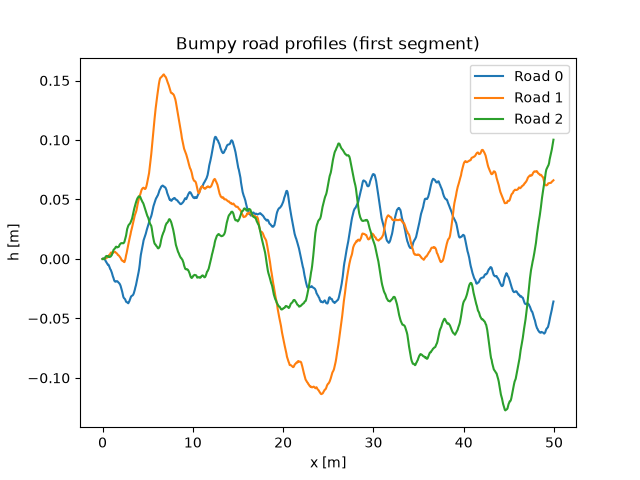
\includegraphics[width=0.48\textwidth]{figures/road_profiles.png}
  \end{center}
\end{frame}

\begin{frame}{Mathematical model}
  General vibration ODE:
  \[
  m u'' + f(u') + s(u) = F(t),
  \qquad u(0)=I,\quad u'(0)=V.
  \]
  \begin{itemize}
    \item Input: mass $m$, damping force $f(u')$, spring force $s(u)$,
          external force $F(t)$, initial data $I$, $V$
    \item Output: vertical displacement $u(t)$
  \end{itemize}
\end{frame}

\begin{frame}{Specialization used in the app}
  In \texttt{bumpy.py} we usually take
  \textbf{linear} spring and damper:
  \[
  m u'' + b u' + k u = F(t).
  \]
  \begin{itemize}
    \item $k$: spring stiffness
    \item $b$: damping coefficient
    \item Typical bicycle defaults:
          $m=60\,\mathrm{kg}$, $k=60\,\mathrm{N/m}$,
          $b=80\,\mathrm{Ns/m}$, $v=5\,\mathrm{m/s}$
  \end{itemize}
  The solver also supports \emph{quadratic} damping
  $f(u') = b|u'|u'$ (see next section).
\end{frame}

\begin{frame}{From road height to forcing}
  Constant speed: $x = v\,t$.
  Vertical acceleration of the road contact:
  \[
  a(t) = \frac{d^2}{dt^2} h(x)
       = v^2\, h''(x).
  \]
  Force on the mass:
  \[
  F(t) = -m\, a(t) = -m\, v^2\, h''(x).
  \]
  So the road curvature (and speed) set the excitation of the suspension.
\end{frame}

\begin{frame}{Animation of the ride}
  \begin{center}
    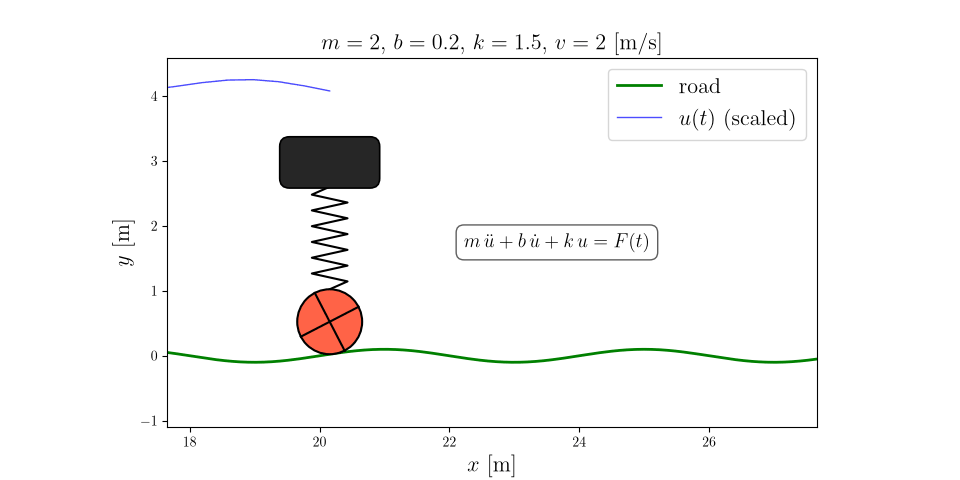
\includegraphics[width=0.75\textwidth]{figures/bumpy_road_still.png}
  \end{center}
  \vspace{0.4em}
  Snapshot from \texttt{bumpy\_road\_anim.py}
  (writes \texttt{bumpy\_road.gif} / \texttt{.mp4} in \texttt{bumpy\_road/}).
\end{frame}

\section{Numerical method}

\begin{frame}{Finite-difference idea}
  \begin{itemize}
    \item Centered differences in time
    \item $u^n$: approximation to $u(t_n)$, $t_n = n\Delta t$
    \item First: linear damping $f(u') = b u'$
  \end{itemize}
\end{frame}

\begin{frame}{Update formula (linear damping)}
  \[
  u^{n+1} =
  \frac{
    2m u^n + \bigl(\tfrac{b}{2}\Delta t - m\bigr) u^{n-1}
    + \Delta t^2\bigl(F^n - s(u^n)\bigr)
  }{
    m + \tfrac{b}{2}\Delta t
  }
  \]
  Special starter step for $n=0$:
  \[
  u^1 = u^0 + \Delta t\, V
  + \frac{\Delta t^2}{2m}\bigl(-b V - s(u^0) + F^0\bigr).
  \]
\end{frame}

\begin{frame}{Quadratic damping}
  For $f(u') = b|u'|u'$, linearize with a geometric mean:
  \[
  |u'|u'\Big|^{n}
  \approx |u'|^{n-\frac12}\,(u')^{n+\frac12}.
  \]
  Resulting update (sketch):
  \[
  u^{n+1}
  = \frac{
    2m u^n - m u^{n-1}
    + b u^n |u^n - u^{n-1}|
    + \Delta t^2\bigl(F^n - s(u^n)\bigr)
  }{
    m + b\,|u^n - u^{n-1}|
  }.
  \]
  Implemented in \texttt{solver.py} via
  \texttt{damping='quadratic'}.
\end{frame}

\begin{frame}[fragile]{Simple linear solver}
  Teaching version: \texttt{solver\_linear\_damping}
  \lstinputlisting[style=pythonTiny]{code/solver_linear.py}
\end{frame}

\begin{frame}[fragile]{Using the linear solver}
  \lstinputlisting[style=pythoncompact]{code/session_linear.py}
  Free vibration: $F\equiv 0$, linear spring $s(u)=2u$.
\end{frame}

\begin{frame}[fragile]{Full solver (API)}
  Improvements over the teaching version:
  \begin{itemize}
    \item linear \emph{and} quadratic damping
    \item $F$ may be a function or a measured array
    \item docstrings; raise exceptions on bad input
  \end{itemize}
\end{frame}

\begin{frame}[fragile]{Full solver (setup and $u^1$)}
  \lstinputlisting[style=pythonTiny]{code/solver_full_part1.py}
\end{frame}

\begin{frame}[fragile]{Full solver (time stepping)}
  \lstinputlisting[style=pythonTiny]{code/solver_full_part2.py}
\end{frame}

\begin{frame}[fragile]{Nonlinear spring + quadratic damping}
  \lstinputlisting[style=pythonTiny]{code/session_quadratic.py}
\end{frame}

\section{Road profiles and forcing}

\begin{frame}[fragile]{Road data as CSV}
  \begin{itemize}
    \item \texttt{draw\_bumpy.csv}: short sample, columns \texttt{x,h}
    \item \texttt{bumpy.csv}: generated file,
          columns \texttt{x,h0,h1,\ldots}
          (several realizations)
  \end{itemize}
  Generate the full file:
\begin{lstlisting}[style=terminal]
uv run python generate_road_profiles.py
uv run python plot_roads.py
\end{lstlisting}
\end{frame}

\begin{frame}{Road profiles}
  \begin{center}
    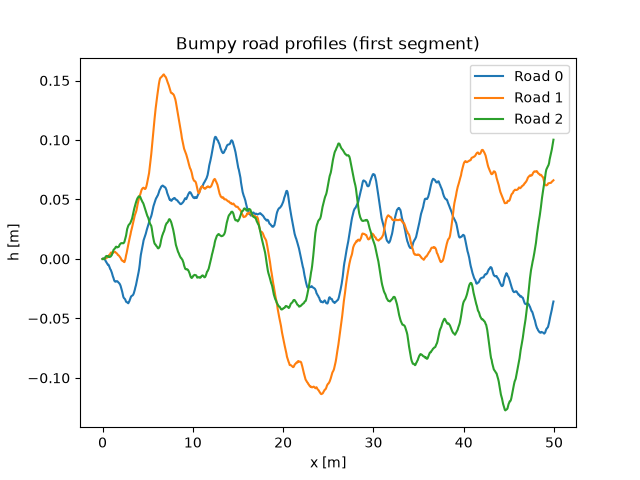
\includegraphics[width=0.70\textwidth]{figures/road_profiles.png}
  \end{center}
\end{frame}

\begin{frame}[fragile]{Loading the CSV}
  \lstinputlisting[style=pythoncompact]{code/load_road_csv.py}
  \begin{itemize}
    \item First column $\to$ distance $x$
    \item Remaining columns $\to$ height profiles
          (rows of \texttt{h\_data})
  \end{itemize}
\end{frame}

\begin{frame}[fragile]{2D array layout (quick reminder)}
\begin{lstlisting}[style=pythoncompact]
>>> h_data.shape          # (nroads, npoints)
(3, 10001)
>>> h = h_data[0, :]      # first road profile
>>> h_data[1, 10:15]      # slice of second profile
\end{lstlisting}
\end{frame}

\begin{frame}{Acceleration from curvature}
  \[
  F(t) \sim -m\, v^2\, h''(x)
  \]
  Approximate $h''(x)$ by centered finite differences on the road mesh.
\end{frame}

\begin{frame}[fragile]{Scalar and vectorized acceleration}
  \lstinputlisting[style=pythonTiny]{code/acceleration.py}
\end{frame}

\begin{frame}[fragile]{Looping over road realizations}
  \lstinputlisting[style=pythoncompact]{code/bumpy_loop.py}
  Resulting list:
  \texttt{[x, t, [h,F,u], [h,F,u], \ldots]}.
\end{frame}

\section{Pipeline and command line}

\begin{frame}{High-level function \texttt{bumpy\_road}}
  \begin{enumerate}
    \item Resolve \texttt{roadfile}: local CSV path or URL
          (\texttt{urllib.request} download if needed)
    \item \texttt{load\_road\_csv} $\to$ $x$, $h$-profiles
    \item Set $t = x/v$; optional stability check on $\Delta t$
    \item For each profile: $a=h''v^2$, $F=-ma$, call \texttt{solver}
    \item Return \texttt{data = [x, t, [h,F,u], \ldots]}
  \end{enumerate}
\end{frame}

\begin{frame}[fragile]{Noise level: RMS displacement}
  \[
  u_{\mathrm{rms}}
  = \sqrt{T^{-1}\int_0^T u^2\,dt}
  \approx
  \sqrt{\frac{1}{N+1}\sum_{n=0}^{N} (u^n)^2}.
  \]
  Compact list comprehension in \texttt{bumpy.py}:
\begin{lstlisting}[style=pythoncompact]
u_rms = [np.sqrt((1.0/len(u))*np.sum(u**2))
         for h, F, u in data[2:]]
\end{lstlisting}
\end{frame}

\begin{frame}[fragile]{Pickling results}
  Persist the whole \texttt{data} list for later plotting:
  \lstinputlisting[style=pythoncompact]{code/pickle_rms.py}
  Use binary modes \texttt{'wb'}/\texttt{'rb'} (Python~3).
\end{frame}

\begin{frame}[fragile]{Command-line options}
  \lstinputlisting[style=pythonTiny]{code/argparse_cli.py}
\end{frame}

\begin{frame}[fragile]{Running a simulation}
\begin{lstlisting}[style=terminal]
uv run python bumpy.py --help
uv run python bumpy.py --v 8 --b 100
uv run python bumpy.py --roadfile bumpy.csv
\end{lstlisting}
  Prints \texttt{u\_rms} values and writes \texttt{bumpy.res}.
\end{frame}

\section{Visual exploration}

\begin{frame}[fragile]{Goals of \texttt{explore.py}}
  After a successful \texttt{bumpy.py} run, plot
  \begin{itemize}
    \item $u(t)$ and $u'(t)$ for $t \ge t_s$
    \item FFT spectra of $u$ and $F$ (dominant frequencies)
    \item stacked panels of $h(x)$, $F(t)$, and $u(t)$
          for each road realization
  \end{itemize}
\begin{lstlisting}[style=terminal]
uv run python explore.py 180
\end{lstlisting}
\end{frame}

\begin{frame}[fragile]{Loading pickled data}
  \lstinputlisting[style=pythoncompact]{code/explore_load.py}
  Boolean mask \texttt{t >= t\_s} selects the late-time window.
\end{frame}

\begin{frame}{Late-time displacement}
  \begin{center}
    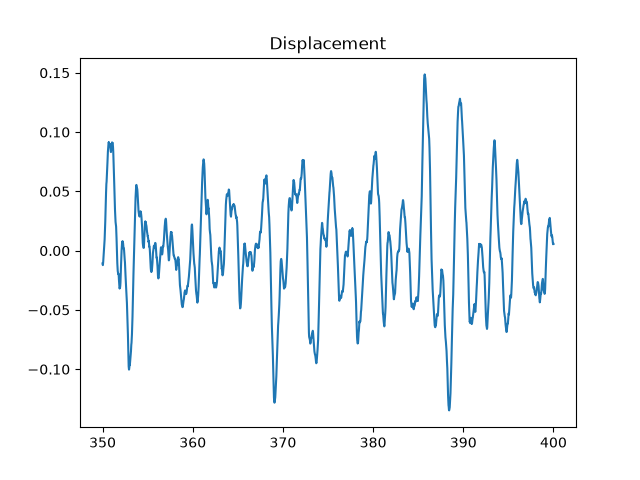
\includegraphics[width=0.72\textwidth]{figures/u1.png}
  \end{center}
\end{frame}

\begin{frame}{Velocity by centered differences}
  \[
  v^n = (u')^n \approx
  \frac{u^{n+1} - u^{n-1}}{2\Delta t}
  \quad (1\le n \le N-1),
  \]
  with one-sided formulas at the ends.
  Vectorized NumPy slicing is much faster than a Python loop.
\end{frame}

\begin{frame}{Velocity plots}
  \begin{columns}[T]
    \begin{column}{0.48\textwidth}
      \centering
      Raw\\
      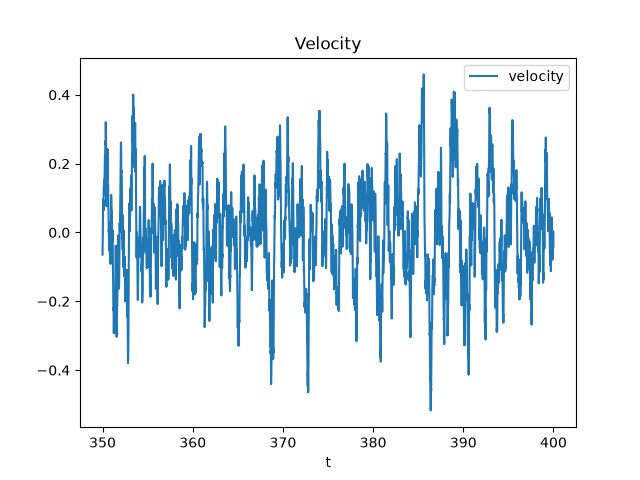
\includegraphics[width=\textwidth]{figures/v1.png}
    \end{column}
    \begin{column}{0.48\textwidth}
      \centering
      Smoothed\\
      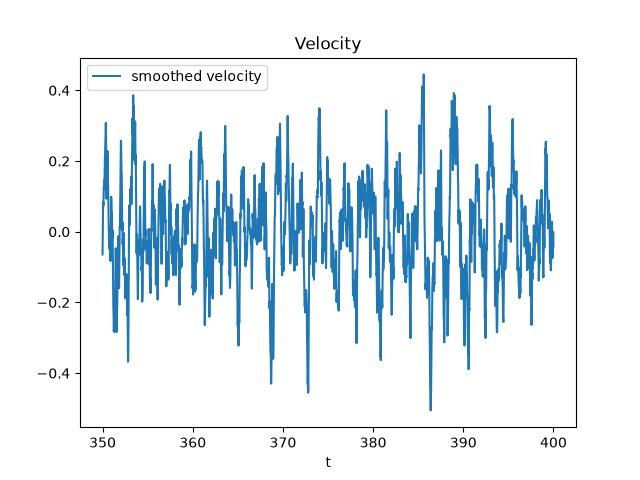
\includegraphics[width=\textwidth]{figures/v1s.png}
    \end{column}
  \end{columns}
\end{frame}

\begin{frame}[fragile]{Frequency analysis (FFT)}
  \lstinputlisting[style=pythonTiny]{code/frequency_analysis.py}
\end{frame}

\begin{frame}{Spectra}
  \begin{center}
    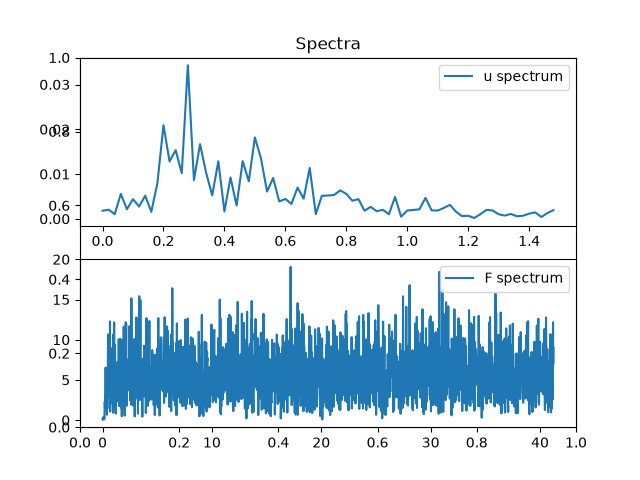
\includegraphics[width=0.68\textwidth]{figures/spectra1.png}
  \end{center}
\end{frame}

\begin{frame}{Road, force, and displacement}
  \begin{center}
    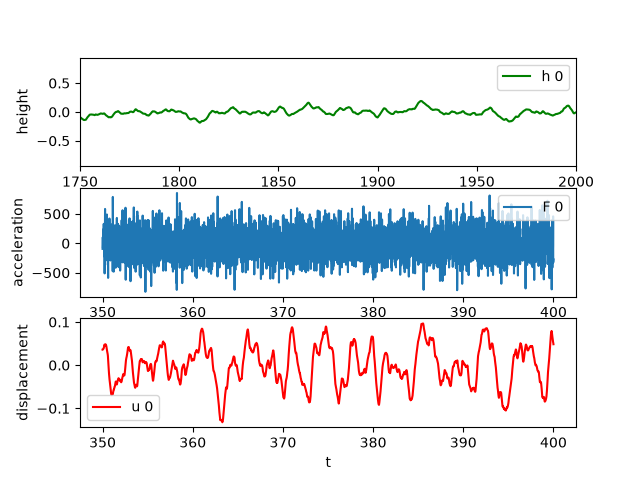
\includegraphics[width=0.62\textwidth]{figures/hFu0.png}
  \end{center}
\end{frame}

\begin{frame}[fragile]{Animation options}
\begin{lstlisting}[style=terminal]
uv run python bumpy_road_anim.py --help
uv run python bumpy_road_anim.py --frames 60 --fps 10
uv run python bumpy_road_anim.py --roadfile draw_bumpy.csv
uv run python bumpy_road_anim.py --roadfile bumpy.csv --profile 0
\end{lstlisting}
  Default road is a built-in sine profile; CSV roads are interpolated.
\end{frame}

\section{Verification and symbolic tools}

\begin{frame}{Why verify?}
  \begin{itemize}
    \item Finite-difference bugs are easy to introduce
    \item A \emph{manufactured solution}: pick a simple exact $u(t)$,
          compute the forcing $F(t)$ that makes the ODE hold,
          then check that the numerical solver recovers $u$
    \item SymPy builds $F$; \texttt{pytest} asserts the error is tiny
  \end{itemize}
\end{frame}

\begin{frame}[fragile]{SymPy sketch of the ODE}
  \lstinputlisting[style=pythoncompact]{code/sympy_demo.py}
  (Modernized Python~3 style; see also \texttt{symbolic.py}
  and \texttt{tests/test\_bumpy.py}.)
\end{frame}

\begin{frame}{Manufactured solution idea}
  Choose e.g.\ $u(t) = I + Vt + qt^2$ (linear damping).
  \begin{enumerate}
    \item Form LHS $= m u'' + b u' + s(u)$ symbolically
    \item Set $F(t) =$ LHS evaluated on that $u$
    \item Call \texttt{solver(..., F, ...)}
    \item Compare numerical $u^n$ to the exact $u(t_n)$
  \end{enumerate}
  For quadratic damping, a linear exact solution
  $u = I + Vt$ is convenient.
\end{frame}

\begin{frame}[fragile]{Test function (excerpt)}
  \lstinputlisting[style=pythonTiny]{code/test_solver.py}
\end{frame}

\begin{frame}[fragile]{Running the tests}
\begin{lstlisting}[style=terminal]
# from the repository root (pyproject.toml)
uv run pytest bumpy_road/tests/test_bumpy.py -q
\end{lstlisting}
  Also covers scalar vs vectorized \texttt{acceleration}.
\end{frame}

\begin{frame}{Optional extras}
  \begin{itemize}
    \item \texttt{--cython} flag in \texttt{bumpy.py}: optional
          compiled solver (not required for the first run)
    \item \texttt{timings.py}: longer runs / performance checks
    \item \texttt{./clean.sh}: remove generated
          \texttt{bumpy.csv}, \texttt{bumpy.res}, plots
  \end{itemize}
\end{frame}

\begin{frame}{Takeaways}
  \begin{itemize}
    \item Road curvature + speed $\to$ forcing of a
          mass--spring--damper ODE
    \item Centered FD time stepping in \texttt{solver.py}
    \item CSV roads, \texttt{uv} workflow, pickle + explore + FFT
    \item Manufactured solutions + \texttt{pytest} for confidence
  \end{itemize}
  \vspace{0.8em}
  Folder: \texttt{bumpy\_road/} in the kinematics repository.
\end{frame}


%%%%%%%%%%%%%%%%%%%
\end{document}
%%%%%%%%%%%%%%%%%%%
